\documentclass[11pt,a4paper]{book}
\usepackage[latin1]{inputenc}
\usepackage{amsmath}
\usepackage{amsfonts}
\usepackage{amssymb}
\usepackage{graphicx}
\usepackage{imakeidx}
% \usepackage{symbols}
\makeindex







\author{Himanshu}
\title{Physics notes}




\begin{document}
\maketitle
\tableofcontents

	
\chapter{Basics}
\section{Basics}
This is some text to get the index working.


$\mu = \nu$
	
$	i\hbar {\frac {\partial }{\partial t}}\Psi (\mathbf {r} ,t)=\left[{\frac {-\hbar ^{2}}{2\mu }}\nabla ^{2}+V(\mathbf {r} ,t)\right]\Psi (\mathbf {r} ,t)$

$E = \frac { 1 } { 2 } N k _ { \mathrm { B } } T$

$F = m \frac { 2 \pi c k _ { \mathrm { B } } T } { \hbar } = m \frac { 4 \pi c } { \hbar } \frac { E } { N } = m \frac { 4 \pi c ^ { 3 } } { \hbar } \frac { M } { N } = m 4 \pi \frac { G M } { A } = G \frac { m M } { r ^ { 2 } }$

$12 \cdot \frac { - i \lambda } { 4 ! } \int d ^ { 4 } z D _ { F } ( x - z ) D _ { F } ( y - z ) D _ { F } ( z - z )$


$\mathcal { L } = \overline { \psi } \left( i \gamma ^ { \mu } \partial _ { \mu } - m \right) \psi - \frac { 1 } { 4 } F _ { \mu \nu } F ^ { \mu \nu } - e \overline { \psi } \gamma ^ { \mu } \psi A _ { \mu }$


\begin{equation}
    \mathcal { L } = \overline { \psi } \left( i \gamma ^ { \mu } \partial _ { \mu } - m \right) \psi - \frac { 1 } { 4 } F _ { \mu \nu } F ^ { \mu \nu } - e \overline { \psi } \gamma ^ { \mu } \psi A _ { \mu }
\end{equation}


\begin{equation}
    \frac { \left\langle 0 _ { + } | \overline { \psi } ( x ) | 0 _ { - } \right\rangle } { \left\langle 0 _ { + } | 0 _ { - } \right\rangle } = \mathrm { i } \int \left( \mathrm { d } x ^ { \prime } \right) \int \frac { \mathrm { d } ^ { 3 } \mathbf { p } } { ( 2 \pi ) ^ { 3 } 2 p ^ { 0 } } \mathrm { e } ^ { - \mathrm { i } p \left( x ^ { \prime } - x \right) } \overline { \eta } \left( x ^ { \prime } \right) ( \gamma p + m )
\end{equation}

\begin{equation}
    \left. \begin{array} { l } { \mathrm { i } \mathrm { W } _ { 21 } = \int \sum _ { \sigma } \frac { m } { p ^ { 0 } } \frac { \mathrm { d } ^ { 3 } \mathbf { p } } { ( 2 \pi ) ^ { 3 } } \left[ \mathrm { i } \overline { \eta } _ { 2 } ( p ) u ( \mathbf { p } , \sigma ) \right] \left[ \mathrm { i } \overline { u } ( \mathbf { p } , \sigma ) \eta _ { 1 } ( p ) \right] } \\ { + \int \sum _ { \sigma } \frac { m } { p ^ { 0 } } \frac { \mathrm { d } ^ { 3 } \mathbf { p } } { ( 2 \pi ) ^ { 3 } } \left[ - \mathrm { i } \overline { v } ( \mathbf { p } , \sigma ) \eta _ { 2 } ( - p ) \right] \left[ - \mathrm { i } \overline { \eta } _ { 1 } ( - p ) v ( \mathbf { p } , \sigma ) \right] } \end{array} \right.
\end{equation}

\begin{equation}
    \left.\begin{aligned} \partial _ { r } & \left[ \sqrt { - g _ { 2 } } \left\{ \left( \rho h + b ^ { 2 } \right) u ^ { r } u _ { \alpha } - b ^ { r } b _ { \alpha } + \delta _ { \alpha } ^ { r } \left( P + \frac { b ^ { 2 } } { 2 } \right) \right\} \right] \\& - \frac { 1 } { 2 } \sqrt { - g _ { 2 } } \left[ \left( \rho h + b ^ { 2 } \right) u ^ { \mu } u ^ { \nu } - b ^ { \mu } b ^ { \nu } + \left( P + \frac { b ^ { 2 } } { 2 } \right) g ^ { \mu \nu } \right] \partial _ { \alpha } g _ { \mu \nu } = 0 \end{aligned} \right.
\end{equation}


\begin{equation}
    \left.\begin{aligned} M _ { \mathrm { K } } & = - \frac { 1 } { 4 \pi } \oint _ { \mathcal { H } } d S _ { a } n _ { b } \nabla ^ { a } \xi ^ { b } - \frac { 1 } { 4 \pi } \int _ { \Sigma _ { t } ^ { \prime } } d V n _ { b } \nabla _ { a } \nabla ^ { a } \xi ^ { b } \\ & = - \frac { 1 } { 4 \pi } \oint _ { \mathcal { H } } d S _ { a } n _ { b } \nabla ^ { a } \xi ^ { b } + \frac { 1 } { 4 \pi } \int _ { \Sigma _ { t } ^ { \prime } } d V n _ { b } R _ { a } ^ { b } \xi ^ { a } \\ & = - \frac { 1 } { 4 \pi } \oint _ { \mathcal { H } } d S _ { a } n _ { b } \nabla ^ { a } \xi ^ { b } + 2 \int _ { \Sigma _ { t } ^ { \prime } } d V \left( T _ { a b } - \frac { 1 } { 2 } g _ { a b } T \right) \xi ^ { a } n ^ { b } \end{aligned} \right.
\end{equation}
	
	
\begin{equation}
\left.\begin{aligned} d s ^ { 2 } = & - d \overline { t } ^ { 2 } + d x ^ { 2 } + d y ^ { 2 } + d z ^ { 2 } \\ & + \frac { 2 M r ^ { 3 } } { r ^ { 4 } + a ^ { 2 } z ^ { 2 } } \left( \frac { r ( x d x + y d y ) - a ( x d y - y d x ) } { r ^ { 2 } + a ^ { 2 } } + \frac { z d z } { r } + d \overline { t } \right) ^ { 2 } \end{aligned} \right.    
\end{equation}


\begin{equation}
    \left. \begin{array} { c } { W ^ { ( \mathrm { e } ) } = \int ( \mathrm { d } x ) \frac { \left( E ^ { 2 } - B ^ { 2 } \right) } { 2 } - [ \frac { 1 } { 8 \pi ^ { 2 } } \int ( \mathrm { d } x ) \int _ { 0 } ^ { \infty } \frac { \mathrm { d } s } { s ^ { 3 } } \mathrm { e } ^ { - s m ^ { 2 } } } \\ { \times \left\{ ( s | \mathrm { e } E | \cot s | \mathrm { e } E | ) ( s | \mathrm { e } B | \operatorname { coth } s | \mathrm { e } B | ) + \frac { ( s \mathrm { e } ) ^ { 2 } \left( E ^ { 2 } - B ^ { 2 } \right) } { 3 } - 1 \right\} ] } \end{array} \right.
\end{equation}





\chapter{Cosmology and inflation}

\section{Basics of Cosmology}


\subsection{Homogeneous cosmology}

Assuming that the universe is homogeneous and isotropic, one can derive \index{Friedmann-Robertson-Walker} (FRW)
metric for the spacetime of the universe.


\begin{equation}
\mathrm{d} s^{2}=-\mathrm{d} t^{2}+a^{2}(t)\left(\frac{\mathrm{d} r^{2}}{1-k r^{2}}+r^{2}\left(\mathrm{d} \theta^{2}+\sin ^{2} \theta \mathrm{d} \phi^{2}\right)\right)
\end{equation}




$a(t)$ is a dimensionless(that`s why it usually comes in equations as a ratio) quantity called scale vector. This helps in working with the co-moving coordinates.

$k$ is $0$ for flat, $1$ for positively curved(Sphere) and $-1$ for negatively curved universe (like a hyperbola). $k$ determines the global geometry, the local geometry can still vary.

\begin{equation}
\mathrm{d} s^{2}=-\mathrm{d} t^{2}+a^{2}(t)\left(\mathrm{d} \chi^{2}+\Phi_{k}\left(\chi^{2}\right)\left(\mathrm{d} \theta^{2}+\sin ^{2} \theta \mathrm{d} \phi^{2}\right)\right)
\end{equation}

\begin{equation}
r^{2}=\Phi_{k}\left(\chi^{2}\right) \equiv\left\{\begin{array}{cc}{\sinh ^{2} \chi} & {k=-1} \\ {\chi^{2}} & {k=0} \\ {\sin ^{2} \chi} & {k=+1}\end{array}\right.
\end{equation}



Because of the FRW ansatz the evolution of the universe boils down to just one parameter, $a(t)$.

\begin{equation}
H \equiv \frac{\dot{a}}{a}
\end{equation}

$H$ is called \index{Hubble parameter}, and is positive for an expanding universe. $H$ kind of sets a natural scale in the cosmology world. For example, characteristic time-scale of the homogeneous universe is the Hubble time, $t \sim H^{-1}$ and characteristic length is Hubble length, $d \sim H^{-1}$.


Casual structure is determined by the propagation of light in the universe, $ds^2 = 0$. To study that we define \textbf{conformal time}: 

\begin{equation}
\tau=\int \frac{\mathrm{d} t}{a(t)}
\end{equation}

Which changes the FRW metric into:
\begin{equation}
\mathrm{d} s^{2}=a(\tau)^{2}\left[-\mathrm{d} \tau^{2}+\left(\mathrm{d} \chi^{2}+\Phi_{k}\left(\chi^{2}\right)\left(\mathrm{d} \theta^{2}+\sin ^{2} \theta \mathrm{d} \phi^{2}\right)\right)\right]
\end{equation}




\chapter{QFT}

\section{Spinors}

\begin{equation}
    \sigma _ { 1 } = \left( \begin{array} { c c } { 0 } & { 1 } \\ { 1 } & { 0 } \end{array} \right) , \quad \sigma _ { 2 } = \left( \begin{array} { c c } { 0 } & { - i } \\ { i } & { 0 } \end{array} \right) , \quad \sigma _ { 3 } = \left( \begin{array} { c c } { 1 } & { 0 } \\ { 0 } & { - 1 } \end{array} \right)
\end{equation}

Having two contracted indices does not guarantee that the whole equation will be Lorentz invariant e.g. $\sigma^\mu \partial_\mu+m = 0 $ is not.

The Lorentz generator algebra is:
\begin{equation}
    \left.\begin{aligned} \left[ J _ { i } , J _ { j } \right] & = i \epsilon _ { i j k } J _ { k } \\ \left[ J _ { i } , K _ { j } \right] & = i \epsilon _ { i j k } K _ { k } \\ \left[ K _ { i } , K _ { j } \right] & = - i \epsilon _ { i j k } J _ { k } \end{aligned} \right.
\end{equation}


\begin{equation}
    \Lambda = \exp \left( i \theta _ { i } J _ { i } + i \beta _ { i } K _ { i } \right)
\end{equation}

Or one can use a shorthand notation:

\begin{equation}
    V ^ { \mu \nu } = \left( \begin{array} { c c c c } { 0 } & { K _ { 1 } } & { K _ { 2 } } & { K _ { 3 } } \\ { - K _ { 1 } } & { 0 } & { J _ { 3 } } & { - J _ { 2 } } \\ { - K _ { 2 } } & { - J _ { 3 } } & { 0 } & { J _ { 1 } } \\ { - K _ { 3 } } & { J _ { 2 } } & { - J _ { 1 } } & { 0 } \end{array} \right)
\end{equation}

Which gives $\Lambda _ { V } = \exp \left( i \theta _ { \mu \nu } V ^ { \mu \nu } \right)$. These V satisfy $\left[ V ^ { \mu \nu } , V ^ { \rho \sigma } \right] = i \left( g ^ { \nu \rho } V ^ { \mu \sigma } - g ^ { \mu \rho } V ^ { \nu \sigma } - g ^ { \nu \sigma } V ^ { \mu \rho } + g ^ { \mu \sigma } V ^ { \nu \rho } \right)$.

\section{Dirac equation}

Dirac Matrices:

\begin{equation}
    \gamma ^ { 0 } = \left( \begin{array} { c } { 1 } \\ { 1 } \end{array} \right) , \quad \gamma ^ { i } = \left( \begin{array} { c c } { 0 } & { \sigma _ { i } } \\ { - \sigma _ { i } } & { 0 } \end{array} \right)
\end{equation}

and they satisfy $\left\{ \gamma ^ { \mu } , \gamma ^ { \nu } \right\} = 2 g ^ { \mu \nu }$.


\begin{equation}
    \left( i \gamma ^ { \mu } \partial _ { \mu } - m \right) \psi = 0
\end{equation}


\chapter{Schwartz}

\section{15: The Casimir effect}

\subsection{Main idea}
This chapter showed two important things using the example of a field in a box:
\begin{itemize}
    \item UV divergence i.e. infinite contribution due to the contribution from arbitrarily small frequencies can be dealt by placing a lower cutoff.
    \item During the intermediate calculations we need to work in a finite sized box and at the end we can take the outer box to be of infinite size. This is to avoid getting infinite contributions during the calculations and will not affect the final force. We can avoid this box by using counterterms which are themselves infinite but drop of when we finally calculate anything physical.
\end{itemize}

\begin{itemize}
    \item Casimir force is independent of any regulator as long as 
    \begin{equation}
        \lim _{x \rightarrow \infty} x f^{(j)}(x)=0 \quad \text { and } \quad f(0)=1
    \end{equation}
    \item It is an infrared effect
\end{itemize}

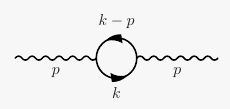
\includegraphics{chapters/QFT/images/image1.png}

\chapter{Path Integrals}


\section{Single particle}

We basically take inspiration from statistical mechanics and try to find equivalent of partition function. (Table 21.1)

Generating functional basically contains all the information that we need, in particular we are mostly concerned about how to find greens functions and $Z[J]$ allows us to do that. Here $J $ is the source function which couples linearly with $\phi(x)$ ,

\begin{equation}
	\mathcal { L } [ \phi ( x ) ] \quad \rightarrow \quad \mathcal { L } [ \phi ( x ) ] + J ( x ) \phi ( x )
\end{equation} again following the analogy with statistical mechanics.

We define:
\begin{equation}
	Z [ J ] = \langle \Omega | \hat { U } ( \infty , - \infty ) | \Omega \rangle _ { J }
\end{equation}

Here $|\Omega \rangle$ denotes the physical ground state and not the free theory ground state.
This denotes the amplitude that we started with no particle and ended up with no particle in presence of a field $J$. i.e. 'No particle  propagator'.

\begin{equation}
	\mathcal { Z } [ J ] = \frac { Z [ J ] } { Z [ J = 0 ] }
\end{equation}


We do this normalization to remove all the vacuum diagrams, which are represented by $Z[J=0]$.

Observe that $U(\infty,-\infty)$ as defined above is not in equal to $\hat{S}$ operator because this is in Heisenberg picture and not in Interaction picture.  Although if we treat the source term as interaction term then we can can at least write $\mathcal { Z } [ J ] = \left\langle \Omega \left| T \mathrm { e } ^ { \mathrm { i } \int \mathrm { d } ^ { 4 } x J ( x ) \hat { \phi } _ { \mathrm { H } } ( x ) } \right| \Omega \right\rangle$ keeping in mind that we still cannot use Wicks theorem. 

Expanding we get:
\begin{equation}
\mathcal { Z } [ J ] = 1 + \sum _ { n = 1 } ^ { \infty } \frac { \mathrm { i } ^ { n } } { n ! } \int \mathrm { d } ^ { 4 } x _ { 1 } \ldots \mathrm { d } ^ { 4 } x _ { n } J \left( x _ { 1 } \right) \ldots J \left( x _ { n } \right) \left\langle \Omega \left| T \hat { \phi } _ { \mathrm { H } } \left( x _ { 1 } \right) \ldots \hat { \phi } _ { \mathrm { H } } \left( x _ { n } \right) \right| \Omega \right\rangle
\end{equation}
And recalling that green's functions are given by:

\begin{equation}
G ^ { ( n ) } \left( x _ { 1 } , \ldots , x _ { n } \right) = \left\langle \Omega \left| T \hat { \phi } _ { \mathrm { H } } \left( x _ { 1 } \right) \ldots \hat { \phi } _ { \mathrm { H } } \left( x _ { n } \right) \right| \Omega \right\rangle
\end{equation}
we get
\begin{equation}
G ^ { ( n ) } \left( x _ { 1 } , \ldots , x _ { n } \right) = \frac { 1 } { \mathrm { i } ^ { n } } \left. \frac { \delta ^ { n } \mathcal { Z } [ J ] } { \delta J \left( x _ { 1 } \right) \ldots \delta J \left( x _ { n } \right) } \right| _ { J = 0 }
\end{equation}
or

\begin{equation}
G ^ { ( n ) } \left( x _ { 1 } , \ldots , x _ { n } \right) = \frac { 1 } { \mathrm { i } ^ { n } } \frac { 1 } { Z [ J = 0 ] } \left. \frac { \delta ^ { n } Z [ J ] } { \delta J \left( x _ { 1 } \right) \ldots \delta J \left( x _ { n } \right) } \right| _ { J = 0 }
\end{equation}

Now we have succeeded in our goal and have a single functional that contains all the information that we require. Now we need to find an automated way of calculating $Z[J]$ and we are done. Two possible ways are:

\begin{enumerate}
\item Relate $ Z[J]$ to S-matrix
\item Use Feynman path integral
\end{enumerate}

\section{Gell-Mann-Low theorem}

What we require to relate our $Z[J]$ to S-matrix is somehow bringing in interaction picture, this is the Gell-Mann-Low theorem:

\begin{equation}
\left\langle \Omega \left| T \hat { \phi } _ { \mathrm { H } } \left( x _ { 1 } \right) \ldots \hat { \phi } _ { \mathrm { H } } \left( x _ { n } \right) \right| \Omega \right\rangle = \frac { \left\langle 0 \left| T \hat { \phi } _ { \mathrm { I } } \left( x _ { 1 } \right) \ldots \hat { \phi } _ { \mathrm { I } } \left( x _ { n } \right) \hat { S } \right| 0 \right\rangle } { \langle 0 | \hat { S } | 0 \rangle }
\end{equation}
Now, if we assume that

\begin{equation}
\mathcal { Z } [ J ] = \frac { Z [ J ] } { Z [ 0 ] } = \frac { \langle 0 | T \mathrm { e } ^ { - \mathrm { i } \int \mathrm { d } ^ { 4 } x [ \hat { \mathcal { H } } _ { I } - J ( x ) \hat { \phi } _ {I } ( x ) ]} | 0 \rangle  } { \langle 0 | T \mathrm { e } ^ { - \mathrm { i } \int \mathrm { d } ^ { 4 } x \mathcal { \hat{H} } _ { I } } | 0 \rangle }
\end{equation}
Which gives:
\begin{equation}
G ^ { ( n ) } \left( x _ { 1 } , \ldots , x _ { n } \right) = \frac { \left\langle 0 \left| T \hat { \phi } _ { \mathrm { I } } \left( x _ { 1 } \right) \ldots \hat { \phi } _ { \mathrm { I } } \left( x _ { n } \right) \hat { S } \right| 0 \right\rangle } { \langle 0 | \hat { S } | 0 \rangle } = \left\langle \Omega \left| T \hat { \phi } _ { \mathrm { H } } \left( x _ { 1 } \right) \ldots \hat { \phi } _ { \mathrm { H } } \left( x _ { n } \right) \right| \Omega \right\rangle
\end{equation}

and we will be done.

Above theorem also gives us the result that 

\begin{equation}
G ^ { ( n ) } = \left\langle \Omega \left| T \hat { \phi } _ { \mathrm { H } } \left( x _ { 1 } \right) \ldots \hat { \phi } _ { \mathrm { H } } \left( x _ { n } \right) \right| \Omega \right) = \sum \left( \begin{array} { c } { \text { All connected diagrams } } \\ { \text { with } n \text { external lines } } \end{array} \right)
\end{equation}

\section{Linked-cluster theorem}
\begin{equation}
\sum \left( \begin{array} { c } { \text { all } } \\ { \text { diagrams } } \end{array} \right) =\mathrm{e}^{ \sum \left( \begin{array} { c } { \text { connected } } \\ { \text { diagrams } } \end{array} \right)}
\end{equation}

This gives us another way of defining what is $Z[J]$, 
\begin{eqnarray*}
Z [ J ] &= &\langle \Omega ( \infty ) | \Omega ( - \infty ) \rangle _ { J } = \langle 0 | \hat { S } | 0 \rangle _ { J }\\
		& =& \sum \left( \begin{array} { c } { \text { Disconnected vacuum and } } \\ { \text { source-to-source diagrams } } 
        \end{array} \right)\\
        &=& { \mathrm { e } }^{\sum \left( \begin{array} { c } { \text { Connected vacuum and } } \\ { \text { source-to-source diagrams } } \end{array} \right)}
\end{eqnarray*}

\section{Path Integrals}

In single particle case we get that amplitude (Probability is thus $\propto |G|^2$) of a particle following a particular path $q(t)$ is:
\begin{eqnarray}
G& =& \int \mathcal { D } [ q ( t ) ] \mathrm { e } ^ { \mathrm { i } \int \mathrm { d } t  \left[ \frac { m \dot{q} ^ { 2 } } { 2 } - V ( q ) \right]} \\
&=& \int \mathcal { D } [ q ( t ) ] \mathrm { e } ^ { \frac { 1 } { \hbar } \int \mathrm { d } t L [ q ( t ) ] } = \int \mathcal { D } [ q ( t ) ] \mathrm { e } ^ { \mathrm { i } S / \hbar }
\end{eqnarray}

Here integration measure is given by:

\begin{equation}
\int \mathcal { D } [ q ( t ) ] = \lim _ { N \rightarrow \infty } \prod _ { n = 1 } ^ { N - 1 } \int \frac { \mathrm { d } q _ { n } } { \xi }
\end{equation}
Observe that paths where $S$ is not stationary i.e.  $\delta S / \delta q ( t ) = 0$ does not hold, we basically end up with zero net contribution due to rapid oscillations in the phase as $\hbar$ is very small. In the limit $\hbar$ goes to zero we get back that classical result.

Gaussian integral:
\begin{eqnarray}
\int _ { - \infty } ^ { \infty } \mathrm { d } x \mathrm { e } ^ { - \frac { a x ^ { 2 } } { 2 }  + b x}& =& \sqrt { \frac { 2 \pi } { a } } \mathrm { e } ^ { \frac { b ^ { 2 } } { 2 a } }\\
\int \mathrm { d } x \mathrm { e } ^ { - x \frac { a } { 2 } x + b x } &= &\sqrt { \frac { 2 \pi } { a } } \mathrm { e } ^ { \frac { 1 } { 2 } \left( b \frac { 1 } { a } b \right) }
\end{eqnarray}

The reason for writing above integrals like this is that generalizations of follow almost same pattern in particular:
\begin{equation}
\mathcal { K } = \int \mathrm { d } ^ { N } x \mathrm { e } ^ { - \frac { 1 } { 2 } \mathbf { x } ^ { \mathrm { T } } \mathbf { A } \mathbf { x } + \mathbf { b } ^ { \mathrm { T } } \mathbf { x } } = \left( \frac { ( 2 \pi ) ^ { N } } { \operatorname { det } \mathbf { A } } \right) ^ { \frac { 1 } { 2 } } \mathrm { e } ^ { \frac { 1 } { 2 } \mathbf { b } ^ { \mathrm { T } } \mathbf { A } ^ { - 1 } \mathbf { b } }
\end{equation}
and,

\begin{equation}
\mathcal { Q } = \int \mathcal { D } [ f ( x ) ] \mathrm { e } ^ { - \frac { 1 } { 2 } \int \mathrm { d } x \mathrm { d } y  f ( x ) A ( x , y ) f ( y ) + \int \mathrm { d } x b ( x ) f ( x ) }=B [det A ( x , y ) ] ^ { - 1 / 2 } e ^ { \frac { 1 } { 2 }  \int \mathrm { d } x \mathrm { d } y b ( x ) A ^ { - 1 } ( x , y ) b ( y )}
\end{equation}
here $A^{-1}(x,y)$ is defined by $\int \mathrm { d } z A ( x , z ) A ^ { - 1 } ( z , y ) = \delta ( x - y )$. And $B$ among other things contains powers of $2\pi $

\textbf{Calculation of above for SHO section 23.3}


\section{Field Integral}

To work with QFT we need fields and not simple paths, we want a functional integral that sums all possible \textit{field configurations} that can exits between the two space-time points.


The generalization stated without proof is simply:

\begin{equation}
\int \mathcal { D } [ \phi ( x ) ] \mathrm { e } ^ { \frac { \mathrm { i } } { 2 }  \int \mathrm { d } ^ { 4 } x \mathrm { d } ^ { 4 } y \phi ( x ) A ( x , y ) \phi ( y ) + \mathrm { i } \int \mathrm { d } ^ { 4 } x b ( x ) \phi ( x )} \\= B [ \operatorname { det } A ( x , y ) ] ^ { - \frac { 1 } { 2 } } \mathrm { e } ^ { - \frac { \mathrm { i } } { 2 } \int \mathrm { d } ^ { 4 } x \mathrm { d } ^ { 4 } y b ( x ) A ^ { - 1 } ( x , y ) b ( y ) }
\end{equation}

Again $B$ contains $(2 \pi \iota)^N$ which diverge in the limit N tends to $\infty$ . Final result is that we can write 

\begin{equation}
Z [ J ] = \int \mathcal { D } [ \phi ( x ) ] \mathrm { e } ^ { \mathrm { i } \int \mathrm { d } ^ { 4 } x \left( \mathcal { L } _ { 0 } + \mathcal { L } _ { \mathrm { I } } + J \phi \right) }
\end{equation}
And for a Lagrangian that can be converted into the form $\phi ( x ) A ( x , y ) \phi ( y ) $ (it turns out these lagrangians (quadratic and bi linear) are exactly those that can be diagonalized using canonical quantization, thus called non-interacting) above integral gives us $Z[J]$.

\subsection{Example calculation for scalar field}

\begin{equation*}
\mathcal { L } _ { 0 } = \frac { 1 } { 2 } \left( \partial _ { \mu } \phi \right) ^ { 2 } - \frac { m ^ { 2 } } { 2 } \phi ^ { 2 }
\end{equation*}
Thus the generating functional is:
\begin{equation*}
Z _ { 0 } [ J ] = \int \mathcal { D } \phi \mathrm { e } ^ { \frac { 1 } { 2 } \int \mathrm { d } ^ { 4 } x \left\{ \left( \partial _ { \mu } \phi \right) ^ { 2 } - m ^ { 2 } \phi ^ { 2 } \right\} + \mathrm { i } \int \mathrm { d } ^ { 4 } x J \phi }
\end{equation*}
$Z _ { 0 } $ basically says that we are working with a free theory. To get the above into the required form we use
\begin{equation*}
\int \mathrm { d } ^ { 4 } x \left( \partial _ { \mu } \phi \right) ^ { 2 } = \left[ \phi \left( \partial _ { \mu } \phi \right) \right] _ { - \infty } ^ { \infty } - \int \mathrm { d } ^ { 4 } x \phi \partial ^ { 2 } \phi
\end{equation*}
Here the first term on RHS goes to zero because we assume that fields die at infinity. Thus we get

\begin{equation}
Z _ { 0 } [ J ] = \int \mathcal { D } \phi \mathrm { e } ^ { \frac { 1 } { 2 } \int \mathrm { d } ^ { 4 } x  \phi \left[ - \left( \partial ^ { 2 } + m ^ { 2 } \right) \right] \phi + \mathrm { i } \int \mathrm { d } ^ { 4 } x J \phi}
\end{equation}Which is nothing but:
\begin{equation}
Z _ { 0 } [ J ] = B [ \operatorname { det } A ( x , y ) ] ^ { - \frac { 1 } { 2 } } \mathrm { e } ^ { - \frac { 1 } { 2 } \int \mathrm { d } ^ { 4 } x \mathrm { d } ^ { 4 } y J ( x ) \left[ \mathrm { i } \hat { A } ^ { - 1 } ( x , y ) \right] J ( y ) }
\end{equation}
with notation $\hat { A } = - \left( \partial ^ { 2 } + m ^ { 2 } \right)$ . The reason to introduce this notation is that $\hat{A}^{-1}$ is just Feynman propagator.
\begin{equation}
\mathrm { i } \hat { A } ^ { - 1 } ( x , y ) = \Delta ( x , y ) = \int \frac { \mathrm { d } ^ { 4 } p } { ( 2 \pi ) ^ { 4 } } \frac { \mathrm { ie } ^ { - \mathrm { i } p \cdot ( x - y ) } } { p ^ { 2 } - m ^ { 2 } + \mathrm { i } \epsilon }
\end{equation}

This gives us another simpler way of calculating Feynman propagator. Now there are two diverging quantities here $B$ and $ \operatorname { det } A ( x , y )$ , but both of these are cancelled by normalization factor i.e. $Z[J=0]$ which is $B \operatorname { det } [ \hat { A } ( x , y ) ] ^ { - \frac { 1 } { 2 } }$. Giving us final result 

\begin{equation}
\mathcal { Z } _ { 0 } [ J ] =e ^ { - \frac { 1 } { 2 } \int d ^ { 4 } x d ^ { 4 } y J ( x ) \Delta ( x - y ) J ( y ) }
\end{equation}
Now using the formula for finding green functions we can see that we have reached the correct result as we get $G _ { 0 } ( x , y ) = \Delta ( x , y)$.






\chapter{Introduction}

\section{Cartan's Exterior Differential Forms}


\subsection{Vectors, 1-Forms, and Tensors}

\subsubsection{Two kinds of Vectors}

In curvilinear coordinate system \textit{u} , the coordinate curve $C_{i}$ (a circle for $\theta$ or x-axis for x) through a point p is the curve where all but $\textit{u}^i$ are constants, and where $\textit{u}^i $is used as a parameter.
 
The tangent vector to this curve is $\partial \mathbf { p } / \partial u ^ { i } \text { which we shall abbreviate to } \partial _ { i } \text { or } \partial / \partial u ^ { i }$.

These vectors form a basis for all vectors $R_n$
This is some more text.






\printindex

\end{document}
\makeglossary